\documentclass[10pt,conference,compsocconf]{IEEEtran}

\usepackage[utf8]{inputenc}
\usepackage{amsmath,amssymb,amsthm}
\usepackage{graphicx}
\usepackage{booktabs}
\usepackage{tabularx}
\usepackage[table]{xcolor}
\usepackage{colortbl}
\usepackage{contour}
\contourlength{0.8pt} % thickness of the halo
\usepackage{url}
\ifCLASSOPTIONcompsoc
  \usepackage[nocompress]{cite}
\else
  \usepackage{cite}
\fi
\usepackage{enumitem}
\usepackage{algorithm}
\usepackage{algpseudocode}
\usepackage{pgf-pie}
\usepackage{pgfplots}
\usepgfplotslibrary{dateplot}
\usepgfplotslibrary{units}
\pgfplotsset{compat=1.18}
\usepackage{comment}
\usepackage{capt-of}
\usepackage[obeyclassoptions,mode=buildnew]{standalone}

\usetikzlibrary{arrows.meta, positioning, calc}

% darken the colors a little bit
\definecolor{red}  {rgb}{0.9,0.0,0.0}
\definecolor{green}{rgb}{0.0,0.7,0.0}
\definecolor{blue} {rgb}{0.0,0.0,0.9}

\definecolor{OkabeBlue}{RGB}{0,114,178}
\definecolor{OkabeOrange}{RGB}{213,94,0}
\definecolor{OkabeGreen}{RGB}{0,158,115}
\definecolor{OkabeSky}{RGB}{86,180,233}
\definecolor{OkabeVermilion}{RGB}{230,159,0}

\definecolor{OIblue}{HTML}{0072B2}
\definecolor{OIorange}{HTML}{E69F00}
\definecolor{OIgrey}{HTML}{999999}

\newcommand{\discuss}[1]{\textcolor{blue}{#1}}
\newcommand{\red}[1]{\textcolor{red}{#1}}
\newcommand{\blue}[1]{\textcolor{green}{#1}}
\newcommand{\edited}[1]{\textcolor{blue}{#1}}
\newcommand{\ori}[1]{\textcolor{blue}{Ori: #1}}

\newif\ifshowaradnotes
\showaradnotesfalse
\newcommand{\arad}[1]{%
  \ifshowaradnotes\par\noindent\textcolor{orange}{\textbf{ARAD NOTE:} #1}\par\fi}

\usepackage[most]{tcolorbox}
\pagestyle{plain}
\title{Mitigating DeFi Impermanent Loss through Risk-Aware Pool Screening}
\thispagestyle{empty}
%\author{\IEEEauthorblockN{Anonymous Authors}}

\author{
\IEEEauthorblockN{Arad Kotzer and Ori Rottenstreich}
\IEEEauthorblockA{
Technion %- Israel Institute of Technology
}
}

\begin{document}

\maketitle

\begin{abstract}
Liquidity provision in automated market makers is widely pursued as a passive income strategy. However, impermanent loss (IL) frequently causes it to underperform simple buy-and-hold portfolios. This shortfall arises when pooled token prices diverge, making liquidity provider performance depend jointly on fee compensation, divergence risk, and the persistence of price-ratio shocks. In this paper, we propose a statistical screening framework to evaluate these tradeoffs using distributional measures of pair-level divergence risk rather than isolated token volatility. Applying this framework to 4.5 years of data across eight major Uniswap v3 pools, we construct comprehensive empirical risk profiles. These profiles integrate full-range constant product market maker proxy IL, downside tail bounds, fee velocity, and mean-reversion half-lives. Our findings demonstrate that relative-price co-movement—rather than individual token volatility—drives proxy IL exposure. Meanwhile, fee compensation depends on capital turnover rather than fee tier alone. Recursive calibration further reveals that historical downside risk estimates carry pool-dependent reliability over time. Finally, a same-sample comparison with stylized passive Uniswap v3 simulations confirms that proxy rankings align closely with realized outcomes under full-range and wide passive bands. However, this alignment deteriorates under tight concentration, where range inactivity and one-sided inventory exposure begin to dominate. Overall, the framework provides a transparent first-stage screening layer for comparing pools and holding horizons prior to deploying detailed protocol-specific range-selection or rebalancing models.
\end{abstract}


\begin{IEEEkeywords}
Blockchain, DeFi, Impermanent Loss
\end{IEEEkeywords}

% \pagestyle{plain}
% \thispagestyle{empty}

\section{Introduction}

The Decentralized Finance (DeFi) ecosystem comprises various financial services that run as blockchain applications~\cite{schar2021decentralized, zetzsche2020decentralized, jensen2021introduction, Bitcoin, wood2014ethereum}. DeFi enables participants to earn yield by providing services. The core strategies revolve around lending money for interest and providing liquidity to token exchanges for transaction fees. They also include generating actions on DeFi platforms to earn engagement rewards. Recent estimates of the DeFi token market cap range from approximately 90 billion USD~\cite{forbes2025defi} to 103 billion~\cite{coingecko2025defi}, as of December 2025.

However, the prevailing narrative that liquidity provision is a passive yield farming strategy is increasingly challenged by the reality of \textit{Impermanent Loss} (IL). IL represents the shortfall between the value of the pool position of a Liquidity Provider (LP) and the value of simply holding the same tokens (HODL). When the relative price of the two assets moves away from its initial level, the Automated Market Maker (AMM) automatically adjusts the pool’s reserve composition to satisfy its pricing rule. 
By doing so, it sells the outperforming asset and buys the underperforming one. 
As a result, the LP's total position value can end up below what they would have obtained by simply holding the assets outside the pool.

Empirical evidence suggests that for many LPs, the fee income generated is insufficient to compensate for this structural drag. 
Loesch et al.~\cite{loesch2021impermanent} study 17 popular Uniswap v2 pools and show that total fees earned (199M USD) failed to offset IL, resulting in an aggregate underperformance of 61M USD compared to the potential revenue of the HODL strategy (261M USD). 
These results imply a yield trap, as headline APYs look attractive, though after subtracting IL, fees often don’t cover the loss.

In this paper, \textit{we present a statistical framework for risk-aware LP pool screening, weighing observed fee compensation against distributional measures of inventory-divergence risk}. 
We operationalize this framework using a full-range CPMM divergence-risk proxy computed from observed price ratios, and then examine its scope through stylized passive Uniswap v3 simulations.
The proposed metrics are intended as a general LP screening layer for AMM environments in which fee compensation must be evaluated against inventory-divergence risk.
We analyze eight major Uniswap v3 pools over 4.5 years to characterize the stochastic behavior of price divergence. 
We focus empirically on Uniswap v3 as it is widely used and because concentrated liquidity provides a demanding setting in which to test when full-range proxy metrics remain informative.
While prior studies focus on theoretical derivation, we introduce actionable, data-driven metrics to support decision-making under uncertainty.

Our analysis reveals that pools fall into distinct risk tiers driven by asset correlation rather than absolute volatility. We show that volatile--volatile pairs often exhibit lower IL risk than stable--volatile pairs due to high correlation. Based on these findings, we derive operational rules for pool selection, showing that maximizing fee velocity and matching horizons to statistical half-lives better predict net profit than the fee tier alone.
We further evaluate the proxy rankings using stylized passive Uniswap v3 simulations with fixed price bands, showing how pool-level screening metrics relate to realized outcomes once concentrated-liquidity mechanics are introduced. 
Table~\ref{tab:notation} summarizes the main notation used throughout the paper.



\begin{table}[t]
\centering
\caption{Summary of notation.}
\label{tab:notation}
\scriptsize
\begingroup
\setlength{\tabcolsep}{3pt}
\renewcommand{\arraystretch}{0.92}
\begin{tabular}{@{}p{0.35\columnwidth}p{0.59\columnwidth}@{}}
\toprule
Notation & Description \\
\midrule
$p_t$, $h$, $R_t^{(h)}$
& Pool price, holding horizon, and normalized price ratio. \\

$\mu_{R^{(h)}}$, $\sigma_{R^{(h)}}$
& Mean and standard deviation of the price ratios. \\

$Z_t^{(h)}$, $\mu_Z$, $\sigma_Z$
& Log-ratio and its mean and standard deviation. \\

$\mathrm{IL}(R)$
& Full-range CPMM proxy IL. \\

$\mathrm{IL}_{\mathrm{mean}}$,
$\mathrm{IL}_{\mathrm{median}}$
& Mean-based and median-based proxy IL. \\

$\mathrm{IL}_{\sigma\text{-bound}}$,
$\mathrm{IL}_{\mathrm{bound}}$
& Standard-deviation and percentile downside bounds. \\

$\phi$, $\mathrm{HL}$
& AR(1) persistence and mean-reversion half-life. \\

$y_t^{\mathrm{fee}}$, $\mathrm{Net90}$
& Fee yield and tail-adjusted screening score. \\

$p_a$, $p_b$, $\delta$, $L$
& Price-range bounds, range width, and position liquidity. \\

$\Pi_{t_0:t_1}$
& Realized passive-v3 excess return over HODL. \\

\bottomrule
\end{tabular}
\endgroup
\end{table}

\section{Background and Related Work}
\label{sec:background}

\subsection{AMM (Automated Market Maker)}
Automated market makers (AMMs)~\cite{hertzog2017bancor} are decentralized exchange protocols that execute token swaps against liquidity pools according to predefined pricing rules. This paper focuses on the constant-product market maker (CPMM), whose reserves satisfy $x_0x_1=K$, as implemented by Uniswap v2. Uniswap v3 retains the constant-product structure but allows liquidity providers to concentrate liquidity within selected price ranges. Within an active range, a position behaves like a CPMM with virtual reserves, while outside the range it becomes inactive and holds only one of the two tokens. These concentrated-liquidity mechanics are discussed in detail in Section~\ref{subsec:cl_valuation}. Other invariant-based AMM designs include Balancer's weighted geometric-mean model and Curve's stableswap model~\cite{bartoletti2022theory}.

AMMs operate as continuous, on-chain price discovery mechanisms driven by arbitrage flow. Whenever the pool price deviates from external markets, arbitrage restores alignment~\cite{angeris2020improved}. 
Hence, arbitrage creates a stabilizing mechanism and a source of value extraction~\cite{pusceddu2024lean}.
This arbitrage-based alignment sustains on-chain liquidity and also determines value transfers. %Traders may pay \emph{slippage} (execution worse than the pre-trade marginal price), and LPs may incur IL when the post-trade reserve mix underperforms HODL. Moreover, adversarial ordering (front-running, sandwiching~\cite{heimbach2022eliminating, zhou2021high}) can extract value under \emph{maximal extractable value} (MEV) \cite{mazorra2022price, daian2020flash, qin2021mev}.

\subsection{Liquidity Provision}
\label{sec:liquidity-provision}

Liquidity provision refers to users depositing tokens into an AMM pool, enabling traders to swap assets directly against pooled reserves. In return, \textit{liquidity providers} (LPs) receive a proportional share of the pool’s swap fees~\cite{gogol2024sok, chiu2023fragility, saengchote2023decentralized}.
For example, in a pool of Uniswap v2 ETH / USDC, LPs deposit equal values of ETH and USDC. Traders then exchange one asset for the other via the constant product invariant of the pool. This mechanism underpins decentralized exchanges by providing continuous on-chain liquidity without order books.
%Fig.~\ref{fig:pool_illustration} illustrates the liquidity provision flow. First, an LP deposits amounts $(x_0,x_1)$ of assets $(c_0,c_1)$ into the pool. When a trader swaps, the pool balances change along the pricing curve, updating the implied price. Finally, upon withdrawal, the LP receives her new proportional mix of tokens plus the fees accrued to the position.

% \begin{figure}[h]
% \centering
% \resizebox{\linewidth}{!}{%
% \begin{tikzpicture}[
%   >={Stealth[length=3mm]},
%   node distance=2.2cm,
%   pool/.style={rectangle, rounded corners, draw, thick, minimum width=4cm, minimum height=1.6cm, align=center},
%   role/.style={rectangle, draw, rounded corners, minimum width=2.4cm, align=center},
%   lab/.style={font=\footnotesize}
% ]
% % Nodes
% \node[role] (lp) {Liquidity Provider (LP)};
% \node[pool, right=3.6cm of lp] (amm) {AMM Pool\\rebalancing by invariant};
% \node[role, right=3.6cm of amm] (trader) {Trader};

% % LP deposit & LP tokens
% \draw[->, thick] (lp.east) -- node[lab, above] {deposit $x_0, x_1$} (amm.west);
% % \draw[<-, thick] ($(amm.west)+(0, -0.35)$) -- node[lab, below] {mint LP tokens} ($(lp.east)+(0, -0.35)$);

% % Trader swap & fees
% \draw[->, thick] (trader.west) -- node[lab, above] {swap $\Delta x_0 \leftrightarrow \Delta x_1$} (amm.east);
% % \draw[->, thick, shorten >=2pt] ($(amm.east)+(0,-0.35)$) -- ++(0.9, -0.7)
% %   node[lab, right, align=left] {fees accrue\\to pool};

% % Withdraw
% \draw[<-, thick, bend right=20] (lp.south) to node[lab, below, align=center] {withdraw new mix\\($x'_0, x'_1$) + fees} (amm.south);

% % Annotations inside pool
% \node[lab] at ($(amm.north)+(0,0.25)$) {price $P = x_1/x_0$};
% \end{tikzpicture}%
% }
% \caption{Liquidity provision illustration of a constant-product AMM}
% \label{fig:pool_illustration}
% \end{figure}


\subsubsection{Fee microstructure and concentrated liquidity}
AMM protocols differ in how fees interact with liquidity.
In Uniswap v2, swap fees are \emph{reinvested into the pool reserves} on each trade, so the product $x_0 \cdot x_1{=}K$ grows.
In Uniswap v3, fees are added to the \emph{separate fee counters} of each position and do not change the active liquidity or the reserves until the LP explicitly claims or reinvests them.
Moreover, v3 allows LPs to choose a price band $[p_{-},p_{+}]$ and provide liquidity only inside it.
Let $p_{\text{pool}}$ denote the instantaneous pool price implied by reserves, defined as
$p_{\text{pool}} = x_1/x_0$. 
When $p_{\text{pool}}\in[p_{-},p_{+}]$, the position behaves locally like a Constant Product Market Maker CPMM (Constant Product Market Maker) with ``virtual'' reserves determined by $[p_{-},p_{+}]$ and its liquidity $L$, and it earns fees. 
If price exits this band, the position becomes out of range and is held entirely in a single asset, $c_0$ when $p_{\text{pool}}<p_{-}$ and $c_1$ when $p_{\text{pool}}>p_{+}$. 
In this out-of-range state, the position provides no active liquidity and therefore accrues no fees until the price re-enters the range or the LP rebalances.


\subsection{Impermanent Loss}
\label{sec:background_il}

\emph{Impermanent Loss} (IL) is the fundamental risk for liquidity providers in AMMs. It is the relative underperformance of an LP's pool position versus a passive buy-and-hold (\emph{HODL}) strategy with the same initial assets~\cite{evans2021liquidity, aoyagi2020liquidity}.


\subsubsection{Mechanism and Formalization}
IL arises from the convex payout structure of the AMM invariant. When the relative market price of the pooled tokens changes, arbitrageurs trade against the pool to realign its internal price with external markets. This process forces the AMM to sell the appreciating asset and buy the depreciating asset, systematically reducing the total value of the pool relative to the HODL benchmark.
For a standard CPMM like Uniswap v2, where reserves $x_0, x_1$ satisfy $x_0 \cdot x_1 = K$, Tiruviluamala et al.~\cite{tiruviluamala2022general} derived the canonical closed-form expression for IL as a function of the price ratio change $R = p'/p$:
\begin{equation}
    \mathrm{IL}(R) = \frac{2\sqrt{R}}{1+R} - 1.
    \label{eq:il_canonical}
\end{equation}
This function is always non-positive ($\mathrm{IL} \le 0$) and symmetric with respect to log-returns, implying that LPs incur losses regardless of the direction of price divergence. While the loss is referred to as impermanent because it theoretically vanishes if prices return to their initial ratio (namely, $IL(R)=0$ for $R=1$), the path-dependent nature of volatility often crystallizes these losses upon withdrawal.

\subsubsection{Empirical Severity}
Empirical studies confirm that $IL \le 0$ is a pervasive feature of AMM liquidity provision, while the ability of fees to offset it depends on pool type and market conditions. 
For Uniswap v2, stablecoin pairs tend to exhibit mild IL, whereas volatile or exotic pairs often experience IL that exceeds fee income~\cite{heimbach2021behavior, boueri2021g3m}. 
In Uniswap v3, concentrated liquidity can amplify divergence exposure, and passive narrow-range positions in volatile pools frequently realize net losses~\cite{heimbach2022risks}. 
Fee-aware analyses report that small price fluctuations can yield impermanent gain when fee flow is sufficiently strong, but this cushioning is limited under large divergence moves~\cite{roman2025impact}.


\subsection{Related Work}
Prior work studies LP risk in AMMs through IL theory and empirical evaluations across protocols.
Canonical results derive closed-form IL for constant-product pools and extend it to broader invariant-based and multi-asset AMM designs~\cite{tiruviluamala2022general}.
Measured underperformance depends on the chosen benchmark and, in Uniswap v3, on concentrated-liquidity mechanics, which make outcomes range-dependent and may leave positions out of range~\cite{aigner2021uniswap,loesch2021impermanent,heimbach2022risks}.
Related perspectives replace HODL with rebalancing-based benchmarks, such as loss-versus-rebalancing (LVR), and derive the fee levels required to compensate LPs fairly~\cite{milionis2022quantifying,milionis2022automated,cohen2023inefficiency}.
Recent work further shows that accounting for fees can materially change conclusions about LP profitability~\cite{roman2025impact} and introduces relative value and fee-adjusted relative value measures for comparing outcomes across AMM designs~\cite{tangri2023generalizing}.


\section{Proxy-Based Statistical Metrics}
\label{sec:metrics}

Section~\ref{sec:background_il} defines IL as a function of the realized relative-price change. Because this change is uncertain when liquidity is supplied, we use historical data to summarize typical outcomes, downside risk, and shock persistence. These quantities are \emph{ex-ante screening proxies}: They provide a common full-range CPMM benchmark for comparing pair-level divergence risk before selecting a concentrated-liquidity range. They do not exactly value a realized Uniswap v3 position or incorporate strategy-specific choices such as band width, rebalancing, and out-of-range management. Section~\ref{sec:empirical_analysis} later tests whether the resulting rankings remain informative under a stylized Uniswap v3 simulation.

{We employ three complementary proxy metrics that capture distinct aspects of divergence risk:}
\begin{enumerate}
    \item \textbf{{Mean-Variance Proxy:}} {Uses standard deviation to define typical risk boundaries under a common full-range benchmark.}
    \item \textbf{{Tail-Risk Proxy (5--95\%) Analysis:}} {Captures adverse divergence episodes using non-parametric quantiles.}
    \item \textbf{{Mean-Reversion Proxy:}} {Estimates the persistence of price-ratio shocks and serves as a horizon-management signal.}
\end{enumerate}

{Since these screening metrics are horizon-specific, we fix a holding horizon length $h$ (e.g., days, weeks, months) and define the corresponding $h$-period normalized price ratio by}
\(
    R^{(h)}_{t} \;=\; \frac{p_{t+h}}{p_t},
\)
{for each feasible start time $t$. Unless stated otherwise, we compute $\{R^{(h)}_{t}\}$ on a rolling basis, so consecutive ratios overlap in time rather than forming disjoint blocks. The proxy metrics below are computed from the empirical distribution $\mathcal{H}_{R^{(h)}}$ induced by the historical series $\{R^{(h)}_{t}\}$.}

\subsection{Mean and Standard Deviation Analysis}
We first characterize the empirical distribution $\mathcal{H}_{R^{(h)}}$ through its sample mean $\mu_{R^{(h)}}$ and sample standard deviation $\sigma_{R^{(h)}}$. Both quantities are horizon-specific and are computed from the rolling $h$-period price ratios defined above. They follow the mean--variance paradigm used in finance~\cite{markowitz1952portfolio,ross2014introduction}.
We map the historical mean $h$-period price ratio to the full-range CPMM formula:
\begin{equation}
\label{eq:il_mean}
\mathrm{IL}_{\text{mean}} = \frac{2\sqrt{\mu_{R^{(h)}}}}{1+\mu_{R^{(h)}}} - 1.
\end{equation}

We note that as $\mathrm{IL}$ is nonlinear, in general
$\mathbb{E}[\mathrm{IL}(R^{(h)})] \neq \mathrm{IL}(\mathbb{E}[R^{(h)}])$.
We use $\mathrm{IL}(\mu_{R^{(h)}})$ only as a comparable ratio-space screening statistic. Dispersion and downside risk are quantified separately.

To obtain a risk interval that contains only strictly positive price ratios, we work in log-ratio space. For each observed $h$-period price ratio $R_i^{(h)}$, we define
\[
Z_i^{(h)}=\ln R_i^{(h)},
\]
and compute the sample mean $\mu_Z$ and sample standard deviation $\sigma_Z$ across these log-ratios. The one-standard-deviation interval in log space is $[\mu_Z-\sigma_Z,\mu_Z+\sigma_Z]$. Transforming its endpoints back to price-ratio space yields $[\exp(\mu_Z-\sigma_Z),\exp(\mu_Z+\sigma_Z)]$. We define the standard-deviation-based IL boundary, $\mathrm{IL}_{\sigma\text{-bound}}$, by evaluating the IL function at the two endpoints:

\begin{equation}
\label{eq:il_sigma_bound}
\resizebox{\linewidth}{!}{$%
\mathrm{IL}_{\sigma\text{-bound}}
= \min\Biggl(
\frac{2\sqrt{\exp(\mu_{Z} - \sigma_{Z})}}{1+\exp(\mu_{Z} - \sigma_{Z})} - 1,\;
\frac{2\sqrt{\exp(\mu_{Z} + \sigma_{Z})}}{1+\exp(\mu_{Z} + \sigma_{Z})} - 1
\Biggr).
$}
\end{equation}

This compact summary is most informative when $\mathcal{H}_{R^{(h)}}$ is reasonably well behaved. Because financial returns can exhibit skewness and heavy tails~\cite{mandelbrot2004fractals}, we also use a non-parametric tail metric.

\subsection{The 5--95 Percentile Metric}

To avoid distributional assumptions and reduce sensitivity to outliers, we identify the fixed 5th and 95th percentiles of $\mathcal{H}_{R^{(h)}}$, denoted $R^{(h)}_{0.05}$ and $R^{(h)}_{0.95}$.
{Using the same common full-range CPMM benchmark, we define the corresponding downside proxy, $\mathrm{IL}_{\text{bound}}$, as the more adverse (most negative) IL value at these percentile extremes:}
\begin{equation}
\label{eq:il_bound}
\mathrm{IL}_{\text{bound}} = \min\left(
\frac{2\sqrt{R^{(h)}_{0.05}}}{1+R^{(h)}_{0.05}} - 1,\quad
\frac{2\sqrt{R^{(h)}_{0.95}}}{1+R^{(h)}_{0.95}} - 1
\right).
\end{equation}

{This construction yields a downside screening threshold such that, in 90\% of observed $h$-period outcomes, the full-range proxy IL is not worse than $\mathrm{IL}_{\text{bound}}$. It therefore summarizes adverse relative-price divergence without requiring a commitment to a specific concentrated-liquidity range.}

Furthermore, we approximate the typical IL by using the median of \(\mathcal{H}_{R^{(h)}}\), denoted \(R^{(h)}_{\text{median}}\). The median-approximated IL is:
\begin{equation}
\label{eq:il_median}
\mathrm{IL}_{\text{median}} = \frac{2\sqrt{R^{(h)}_{\text{median}}}}{1+R^{(h)}_{\text{median}}} - 1.
\end{equation}

{To quantify sampling uncertainty in this non-parametric summary, we report a 95\% confidence interval for $\mathrm{IL}_{\text{median}}$ in the empirical section. This directly addresses the instability of point estimates in relatively short monthly samples and makes the screening layer more statistically transparent.}

\subsection{Mean-Reversion-Based Predictability Metric}
\label{subsubsec:mean_reversion_metric}

Finally, we capture how long relative-price shocks persist. Magnitude alone does not distinguish a quickly reverting divergence from one that can remain throughout the LP's holding period. Before estimating persistence, we perform an Augmented Dickey--Fuller (ADF) test as a stationarity diagnostic for the log price-ratio series.

Let \(R_t\) denote the oriented price ratio sampled at the chosen frequency, and define the log-ratio \(Z_t = \ln R_t\).
We model \(Z_t\) with a basic mean-reverting model that describes how deviations from a long-run level \(\mu\) evolve over time:
\begin{equation}
\label{eq:ar1_ratio}
Z_{t+1} - \mu = \phi \bigl(Z_t - \mu\bigr) + \varepsilon_{t+1}, 
\qquad \varepsilon_{t+1} \stackrel{\mathrm{i.i.d.}}{\sim} N(0, \sigma^2_\varepsilon).
\end{equation}
Here, $0<\phi<1$ controls how quickly deviations decay, and $\varepsilon_{t+1}$ captures new information. Values near one imply slower adjustment.

We interpret this AR(1) specification as a reduced-form persistence proxy rather than a structural model of AMM dynamics. It summarizes the persistence of pair-level relative-price shocks and provides a simple horizon-management signal for the screening layer. In the empirical analysis, we report point estimates of $\hat{\phi}$ and the corresponding mean-reversion half-life.

A convenient way to express the speed of reversion is the \emph{half-life} ($HL$), defined as the number of periods required for a deviation in $Z_t$ to decay by 50\%. For the AR(1) process $Z_t-\mu=\phi(Z_{t-1}-\mu)+\varepsilon_t$, with $0<\phi<1$, the
half-life is
\[
HL=-\frac{\ln 2}{\ln\phi}.
\]
We exclude windows for which $\hat{\phi}\notin(0,1)$, since a positive mean-reversion half-life is then undefined. A shorter $HL$ indicates faster dissipation of relative-price shocks. Thus, $HL$ provides a horizon-management signal for matching intended LP holding horizons to the estimated persistence of divergence risk.

\subsection{Tail-Adjusted Screening Metric (Net90)}
\label{subsec:net90}

The proxy metrics above summarize complementary aspects of pair-level divergence risk under the common full-range benchmark. In practice, however, pool screening also requires incorporating the fee side of liquidity provision. A pool with mild divergence risk may still be unattractive if fee generation is too weak, while a pool with stronger fee flow may remain viable despite moderate downside exposure. This motivates a simple tail-adjusted screening score that combines fee income with an adverse IL scenario.

Let $y^{\text{fee}}_t$ denote the realized fee yield over the chosen horizon and let $\mathrm{IL}_t$ denote the corresponding proxy IL realization under the common full-range benchmark. We define the \emph{Tail-Adjusted Yield} (\emph{Net90}) as
\begin{equation}
\label{eq:net90}
\mathrm{Net90}
=
\operatorname{median}\!\left(y^{\text{fee}}_{t}\right)
+
\operatorname{P}_{10}\!\left(\mathrm{IL}_{t}\right),
\end{equation}
where $\operatorname{P}_{10}(\mathrm{IL}_t)$ is the 10th percentile of the proxy-IL distribution across historical horizon-level observations.

Net90 is designed as an \emph{ex-ante screening score}. The first term captures the typical fee income available in the pool, while the second term imposes a downside adjustment based on a 90th-percentile adverse divergence event. Because $\mathrm{IL}_t \le 0$, the second term penalizes pools whose fee income is not sufficient to absorb large relative-price dislocations. Higher Net90 values therefore indicate pools whose structural fee generation remains more robust after accounting for tail divergence risk.

This metric should not be interpreted as an exact forecast of realized Uniswap v3 profitability under concentrated liquidity. Rather, like the other metrics presented above, it is a strategy-agnostic screening device under a common benchmark. Its role is to rank pools ex ante before specifying a particular concentrated-liquidity policy. In Section~\ref{sec:empirical_analysis}, we use Net90 as the main cross-pool screening score and then test whether the resulting ranking remains informative under stylized passive Uniswap v3 strategies.


\subsection{{Stylized Concentrated-Liquidity Valuation}}
\label{subsec:cl_valuation}

Actual Uniswap v3 positions are range-dependent and earn fees only while active. We therefore introduce a stylized concentrated-liquidity valuation layer to test whether the proxy rankings remain informative under fixed passive bands. It is a controlled validation setting rather than a model of active LP management.

{We consider a passive LP who enters a position at time $t_0$ when the pool price is $p_0$, chooses a fixed price range $[p_a,p_b]$, and holds the position until horizon end $t_1$ without rebalancing. In the empirical analysis, we study symmetric bands around the entry price, so that $p_a=(1-\delta)p_0$ and $p_b=(1+\delta)p_0$, where $\delta$ denotes the chosen concentration width. We evaluate several stylized widths, together with a full-range benchmark. We assume the LP provides liquidity passively, with no range updates, no fee compounding, and no transaction costs.}

{Let $L$ denote the liquidity parameter of the position. For a given terminal price $p_1$, the terminal inventory depends on whether the final price lies below, within, or above the selected range. Expressed in the numeraire of token~1, the terminal mark-to-market value of the position is given by the standard piecewise concentrated-liquidity formula}
\begin{equation}
\label{eq:v3_terminal_value}
V^{\mathrm{pos}}_1(p_1)=
\begin{cases}
L\left(\dfrac{1}{\sqrt{p_a}}-\dfrac{1}{\sqrt{p_b}}\right)p_1, & p_1 < p_a,\\[1.0em]
L\left(2\sqrt{p_1}-\sqrt{p_a}-\dfrac{p_1}{\sqrt{p_b}}\right), & p_a \le p_1 \le p_b,\\[1.0em]
L\left(\sqrt{p_b}-\sqrt{p_a}\right), & p_1 > p_b.
\end{cases}
\end{equation}

{This representation captures the defining feature of concentrated liquidity: When price exits the chosen band, the LP position is fully converted into a single asset and no longer behaves like an active two-sided liquidity position. As a consequence, both valuation and fee accrual become path-dependent.}

{To initialize the position, we normalize the LP’s entry wealth to a fixed notional $V_0$, identical across pools and strategy widths. Given the entry price $p_0$ and the chosen band $[p_a,p_b]$, this notional determines the implied liquidity $L$. This normalization ensures that realized outcomes are directly comparable across pools and concentration widths. As a benchmark, we compare the LP position against a passive HODL portfolio formed from the same initial token amounts at entry.}

{Unlike the ex-ante proxy metrics above, the concentrated-liquidity layer is evaluated on a daily path. For each day $t \in [t_0,t_1]$, we mark the LP position to market using the prevailing price $p_t$ and determine whether the position is active, i.e., whether $p_t \in [p_a,p_b]$. Fee income is accrued only on days when the position is in range. Because our dataset is pool-level rather than position-level, exact reconstruction of active-liquidity shares at each tick is not available. We therefore approximate daily fee income by allocating a fraction of the pool’s daily fees to the stylized LP conditional on the position being in range. This approximation should be interpreted as a reduced-form passive fee rule rather than an exact wallet-level accounting of realized Uniswap v3 fee claims.}

{Formally, let $y^{\mathrm{fee}}_t$ denote the daily fee income assigned to the stylized LP and let $\mathbf{1}\{p_t \in [p_a,p_b]\}$ be the indicator that the position is active on day $t$. The cumulative fee income over the holding horizon is then}
\begin{equation}
\label{eq:cum_fee_income}
Y^{\mathrm{fee}}_{t_0:t_1}
=
\sum_{t=t_0}^{t_1}
y^{\mathrm{fee}}_t \cdot \mathbf{1}\{p_t \in [p_a,p_b]\}.
\end{equation}

{Denoting the HODL terminal value by $V^{\mathrm{HODL}}_1(p_1)$, we define the realized passive concentrated-liquidity excess return over the episode as}
\begin{equation}
\label{eq:passive_v3_profit}
\Pi_{t_0:t_1}
=
\frac{V^{\mathrm{pos}}_1(p_1)+Y^{\mathrm{fee}}_{t_0:t_1}-V^{\mathrm{HODL}}_1(p_1)}{V_0}.
\end{equation}

Unlike the ex-ante proxy metrics, $\Pi_{t_0:t_1}$ is a realized outcome under a specific range. Comparing the two rankings reveals when concentrated liquidity changes the pool ordering. The setup deliberately excludes active repositioning, dynamic optimization, slippage, gas costs, and wallet-level fee reconstruction.



\section{Empirical Analysis on Real Pools}
\label{sec:empirical_analysis}

After presenting the proxy-based screening metrics in Section~\ref{sec:metrics}, we now apply them to real data from eight Uniswap v3 pools. The empirical analysis has two layers. First, we characterize and compare pools using the ex-ante screening proxies introduced in Section~\ref{sec:metrics}. Second, we evaluate whether the resulting rankings remain informative under a stylized passive Uniswap v3 simulation based on concentrated-liquidity valuation and daily path-dependent fee accrual.


\subsection{Data}

% \begin{table}[t]
% \centering
% \scriptsize
% \resizebox{0.5\textwidth}{!}{%
% \begin{tabular}{lll}
% \hline
% Pool address & Tokens & Fee tier\\
% \hline
% \texttt{0x4e68ccd3e89f51c3074ca5072bbac773960dfa36} & WETH/USDT & 0.30\% \\
% \texttt{0x11b815efb8f581194ae79006d24e0d814b7697f6} & WETH/USDT & 0.05\% \\
% \texttt{0x9db9e0e53058c89e5b94e29621a205198648425b} & WBTC/USDT & 0.30\% \\
% \texttt{0x4585fe77225b41b697c938b018e2ac67ac5a20c0} & WBTC/WETH & 0.05\% \\
% \texttt{0xcbcdf9626bc03e24f779434178a73a0b4bad62ed} & WBTC/WETH & 0.30\% \\
% \texttt{0x5ab53ee1d50eef2c1dd3d5402789cd27bb52c1bb} & AAVE/WETH & 0.30\% \\
% \texttt{0xa6cc3c2531fdaa6ae1a3ca84c2855806728693e8} & LINK/WETH & 0.30\% \\
% \texttt{0x1d42064fc4beb5f8aaf85f4617ae8b3b5b8bd801} & UNI/WETH & 0.30\% \\
% \hline
% \end{tabular}
% }
% \caption{Summary of Uniswap v3 pools used in the empirical analysis.}
% \label{tab:pools}
% \end{table}


\begin{table}[t]
\centering
\scriptsize
\resizebox{0.5\textwidth}{!}{%
\begin{tabular}{llll}
\hline
Pool ID & Tokens & Fee tier & Category\\
\hline
\texttt{4e} & WETH/USDT & 0.30\% & Stable--volatile\\
\texttt{11} & WETH/USDT & 0.05\% & Stable--volatile\\
\texttt{9d} & WBTC/USDT & 0.30\% & Stable--volatile\\
\texttt{45} & WBTC/WETH & 0.05\% & Volatile--volatile\\
\texttt{cb} & WBTC/WETH & 0.30\% & Volatile--volatile\\
\texttt{5a} & AAVE/WETH & 0.30\% & Protocol-token\\
\texttt{a6} & LINK/WETH & 0.30\% & Protocol-token\\
\texttt{1d} & UNI/WETH  & 0.30\% & Protocol-token\\
\hline
\end{tabular}
}
\caption{Summary of Uniswap v3 pools used in the empirical analysis. }
\label{tab:pools}
\end{table}

We collect historical data for eight major Uniswap v3 liquidity pools using The Graph's public subgraph\footnote{\url{https://thegraph.com/explorer}}, covering 4.5 years (May~2021--December~2025). For each pool, we extract daily price, fee, and liquidity-related information and construct the normalized price-ratio series used in the proxy layer. The dataset covers two fee tiers (0.05\% and 0.30\%) and three pool categories: (i) Stable--volatile pairs (WETH/USDT and WBTC/USDT), (ii) Volatile--volatile pairs (WBTC/WETH), and (iii) Protocol-token pairs (AAVE/WETH, LINK/WETH, and UNI/WETH). WETH and WBTC denote wrapped Ether and wrapped Bitcoin, respectively. USDT denotes Tether's U.S.-dollar-pegged stablecoin, while AAVE, LINK, and UNI are the tokens associated with the Aave, Chainlink, and Uniswap protocols, respectively.
For reproducibility, we publish the raw data and scripts in a GitHub repository~\cite{mitigation_code}.


The screening metrics above are computed using the standard full-range CPMM formula applied to observed price ratios. We use this as a common pair-level benchmark for divergence risk, enabling consistent comparisons across pools and fee tiers before specifying a concentrated-liquidity strategy. These quantities are therefore ex-ante screening proxies rather than exact valuations of realized Uniswap v3 positions.
The empirical section also goes beyond the proxy layer. Beyond monthly screening, we evaluate stylized passive Uniswap v3 strategies using daily path-dependent simulation under fixed price bands. This second layer allows us to test whether pools favored by simpler proxy metrics also perform well under concentrated liquidity.
We evaluate screening results at a one-month horizon. This interval matches a natural monitoring and repositioning frequency for LPs and yields enough observations over 4.5 years to estimate cross-pool risk summaries. By contrast, daily horizons are noisy and dependent, while annual horizons yield too few samples for stable estimation.



% \begin{figure}[t]
% \centering
% \resizebox{0.5\textwidth}{!}{%
%     \begin{tikzpicture}
  \begin{axis}[
    width=0.95\linewidth,
    height=0.7\linewidth,
    xlabel={Month},
    ylabel={Total Value Locked (USD)},
    xmin=1, xmax=56,
    ymode=log,
    ymin=1e5, ymax=1e9,
    ymajorgrids=true,
    xmajorgrids=false,
    xtick={1,13,25,37,49},
    xticklabels={2021-05,2022-05,2023-05,2024-05,2025-05},
    xticklabel style={
        font=\scriptsize,
        rotate=35,
        anchor=east
    },
    xlabel style={yshift=-0.5em},
    legend style={at={(0.02,0.02)},anchor=south west,font=\tiny,draw=black,fill=white,fill opacity=0.9,text opacity=1},
    legend cell align=left,
]

    % Data file: tvl_analysis/tvl_monthly_end.dat
    % Expected columns: month tvl_45 tvl_cb tvl_4e tvl_11 tvl_9d tvl_5a tvl_a6 tvl_1d

    % 45: WBTC/WETH 0.05%
    \addplot+[
      color=blue!85!black,
      mark=x,
      line width=0.8pt
    ] table[x=month,y=tvl_45] {tvl_analysis/tvl_monthly_end.dat};
    %\addlegendentry{45: WBTC/WETH 0.05\%}

    % cb: WBTC/WETH 0.30%
    \addplot+[
      color=blue!35!white,
      mark=pentagon*,
      mark options={fill=blue!35!white},
      line width=0.8pt
    ] table[x=month,y=tvl_cb] {tvl_analysis/tvl_monthly_end.dat};
    %\addlegendentry{cb: WBTC/WETH 0.30\%}

    % 4e: WETH/USDT 0.30%
    \addplot+[
      color=green!60!black,
      mark=*,
      mark options={fill=green!60!black},
      line width=0.8pt
    ] table[x=month,y=tvl_4e] {tvl_analysis/tvl_monthly_end.dat};
    %\addlegendentry{4e: WETH/USDT 0.30\%}

    % 11: WETH/USDT 0.05%
    \addplot+[
      color=green!25!black,
      mark=diamond*,
      mark options={fill=green!25!black},
      line width=0.8pt
    ] table[x=month,y=tvl_11] {tvl_analysis/tvl_monthly_end.dat};
    %\addlegendentry{11: WETH/USDT 0.05\%}

    % 9d: WBTC/USDT 0.30%
    \addplot+[
      color=violet!75!black,
      mark=triangle*,
      mark options={fill=violet!75!black},
      line width=0.8pt
    ] table[x=month,y=tvl_9d] {tvl_analysis/tvl_monthly_end.dat};
    %\addlegendentry{9d: WBTC/USDT 0.30\%}

    % 5a: AAVE/WETH 0.30%
    \addplot+[
      color=purple!75!black,
      mark=square*,
      mark options={fill=purple!75!black},
      dashed,
      line width=0.8pt
    ] table[x=month,y=tvl_5a] {tvl_analysis/tvl_monthly_end.dat};
    %\addlegendentry{5a: AAVE/WETH 0.30\%}

    % a6: LINK/WETH 0.30%
    \addplot+[
      color=orange!85!black,
      mark=star,
      mark options={fill=orange!85!black},
      line width=0.8pt
    ] table[x=month,y=tvl_a6] {tvl_analysis/tvl_monthly_end.dat};
    %\addlegendentry{a6: LINK/WETH 0.30\%}

    % 1d: UNI/WETH 0.30%
    \addplot+[
      color=cyan!80!black,
      mark=otimes*,
      mark options={fill=cyan!80!black},
      line width=0.8pt
    ] table[x=month,y=tvl_1d] {tvl_analysis/tvl_monthly_end.dat};
    %\addlegendentry{1d: UNI/WETH 0.30\%}

  \end{axis}
\end{tikzpicture}
% }
% \caption{Pool monthly total value locked (TVL), in USD.}
% \label{fig:monthly_tvl}
% \end{figure}

% \begin{figure}[t]
%     \centering
%     \resizebox{0.5\textwidth}{!}{%
%         \begin{tikzpicture}
  \begin{axis}[
    width=0.95\linewidth,
    height=0.72\linewidth,
    xlabel={Month},
    ylabel={Trading Volume (USD)},
    xmin=1, xmax=56,
    ymode=log,
    ymin=1e6, ymax=3e10,
    ymajorgrids=true,
    xmajorgrids=false,
    xtick={1,12,23,34,45,56},
    xticklabels={2021-05,2022-04,2023-03,2024-02,2025-01,2025-12},
    xticklabel style={
        font=\scriptsize,
        rotate=35,
        anchor=east
    },
    xlabel style={yshift=-0.5em},
    legend style={at={(0.02,0.02)},anchor=south west,font=\tiny,draw=black,fill=white,fill opacity=0.9,text opacity=1},
    legend cell align=left,
]

    % Data file: trading_volume/trading_volume_monthly.dat
    % Expected columns: month vol_45 vol_cb vol_4e vol_11 vol_9d vol_5a vol_a6 vol_1d

    % 45: WBTC/WETH 0.05%
    \addplot+[
      color=blue!85!black,
      mark=x,
      line width=0.8pt
    ] table[x=month,y=vol_45] {trading_volume/trading_volume_monthly.dat};
    %\addlegendentry{45: WBTC/WETH 0.05\%}

    % cb: WBTC/WETH 0.30%
    \addplot+[
      color=blue!35!white,
      mark=pentagon*,
      mark options={fill=blue!35!white},
      line width=0.8pt
    ] table[x=month,y=vol_cb] {trading_volume/trading_volume_monthly.dat};
    %\addlegendentry{cb: WBTC/WETH 0.30\%}

    % 4e: WETH/USDT 0.30%
    \addplot+[
      color=green!60!black,
      mark=*,
      mark options={fill=green!60!black},
      line width=0.8pt
    ] table[x=month,y=vol_4e] {trading_volume/trading_volume_monthly.dat};
    %\addlegendentry{4e: WETH/USDT 0.30\%}

    % 11: WETH/USDT 0.05%
    \addplot+[
      color=green!25!black,
      mark=diamond*,
      mark options={fill=green!25!black},
      line width=0.8pt
    ] table[x=month,y=vol_11] {trading_volume/trading_volume_monthly.dat};
    %\addlegendentry{11: WETH/USDT 0.05\%}

    % 9d: WBTC/USDT 0.30%
    \addplot+[
      color=violet!75!black,
      mark=triangle*,
      mark options={fill=violet!75!black},
      line width=0.8pt
    ] table[x=month,y=vol_9d] {trading_volume/trading_volume_monthly.dat};
    %\addlegendentry{9d: WBTC/USDT 0.30\%}

    % 5a: AAVE/WETH 0.30%
    \addplot+[
      color=purple!75!black,
      mark=square*,
      mark options={fill=purple!75!black},
      dashed,
      line width=0.8pt
    ] table[x=month,y=vol_5a] {trading_volume/trading_volume_monthly.dat};
    %\addlegendentry{5a: AAVE/WETH 0.30\%}

    % a6: LINK/WETH 0.30%
    \addplot+[
      color=orange!85!black,
      mark=star,
      mark options={fill=orange!85!black},
      line width=0.8pt
    ] table[x=month,y=vol_a6] {trading_volume/trading_volume_monthly.dat};
    %\addlegendentry{a6: LINK/WETH 0.30\%}

    % 1d: UNI/WETH 0.30%
    \addplot+[
      color=cyan!80!black,
      mark=otimes*,
      mark options={fill=cyan!80!black},
      line width=0.8pt
    ] table[x=month,y=vol_1d] {trading_volume/trading_volume_monthly.dat};
    %\addlegendentry{1d: UNI/WETH 0.30\%}

  \end{axis}
\end{tikzpicture}

%     }
%     \caption{Pool monthly total trading volume (in USD).}
%     \label{fig:monthly_pools_volume}
% \end{figure}


\subsubsection{Fee velocity across fee tiers}
For the same token pair, arbitrage keeps prices closely aligned across fee tiers, while turnover---volume relative to TVL---can differ substantially.
Because gross fee yield is approximately $y^{\mathrm{fee}}\approx\mathrm{FeeTier}\times\mathrm{Volume}/\mathrm{TVL}$, a 0.05\% pool requires six times the turnover of a 0.30\% pool to match its fee yield, and more than six times to exceed it. In May~2021, WBTC/WETH pool 45 achieved approximately $57\times$ turnover versus $5.4\times$ for pool cb, so its $10.5\times$ turnover advantage produced higher gross fee yield before IL. Conversely, WETH/USDT pool 11 achieved $77\times$ turnover versus $14\times$ for pool 4e; its $5.5\times$ advantage was insufficient to offset the lower fee tier. Pool comparison should therefore consider fee velocity jointly with divergence risk rather than fee tier or raw volume alone.

\subsection{Proxy IL and Net-Loss Episodes}

The descriptive pool statistics above show that the pools differ substantially in price dynamics, liquidity, and trading activity. We next translate the observed monthly price-ratio movements into the full-range proxy IL benchmark introduced in Section~\ref{sec:metrics}. This allows us to compare divergence losses across pools before imposing any particular concentrated-liquidity range policy.

Fig.~\ref{fig:monthly_il} presents monthly full-range proxy IL computed from the observed monthly price ratios. These values should be interpreted as ex-post realizations of the common screening benchmark, not as exact valuations of concentrated-liquidity positions.
The two WETH/USDT pools (4e and 11) incurred the largest proxy IL losses during the mid--2022 drawdown. Their worst month was June~2022, with proxy IL values of $-3.91\%$ and $-3.90\%$, respectively. In contrast, the correlated WBTC/WETH pools (45 and cb) experienced only mild proxy IL losses in June~2022, both approximately $-0.16\%$. However, both experienced a marked divergence episode in mid--2025. Their largest monthly proxy IL losses occurred in July~2025, at approximately $-1.33\%$, consistent with an idiosyncratic BTC--ETH divergence rather than a broad market shock.

The remaining pools fell into an intermediate risk band. WBTC/USDT (9d) and UNI/WETH (1d) recorded proxy IL losses of $-2.56\%$ and $-2.58\%$, respectively, in June~2022. LINK/WETH (a6) reached its largest loss in May~2025, at $-1.69\%$, while AAVE/WETH (5a) reached its largest loss in December~2024, at $-3.24\%$.

\begin{figure}[t]
  \centering
  \begin{tikzpicture}
    \begin{axis}[
      width=0.32\textwidth,
      height=0.2\textheight,
      xmin=1,
      xmax=55,
      % --- UPDATED LIMITS (Scaled by 100) ---
      ymin=-4, 
      ymax=0.1, 
      xlabel={Month},
      ylabel={Monthly IL},
      xticklabel style={rotate=45, anchor=east, font=\tiny},
      xtick=\empty,
      extra x ticks={1,4,7,10,13,16,19,22,25,28,31,34,37,40,43,46,49,52,55},
      extra x tick style={xticklabel style={rotate=45, anchor=east, font=\tiny}},
      extra x tick labels={%
        2021-06,2021-09,2021-12,%
        2022-03,2022-06,2022-09,2022-12,%
        2023-03,2023-06,2023-09,2023-12,%
        2024-03,2024-06,2024-09,2024-12,%
        2025-03,2025-06,2025-09,2025-12},
      scaled y ticks=false,
      % --- DATA FILTER (Multiplies y-values by 100) ---
      y filter/.code={\pgfmathparse{\pgfmathresult*100}\pgfmathresult},
      % --- UPDATED TICKS & LABELS ---
      yticklabel style={/pgf/number format:fixed, /pgf/number format:precision=1},
      yticklabel={\pgfmathprintnumber{\tick}\%}, % Adds the % sign
      ytick={-4,-3.5,-3,-2.5,-2,-1.5,-1,-0.5,0},
      grid=both,
      legend style={
        at={(1.31,0.02)},
        anchor=south,
        legend columns=1,
        font=\tiny,
        draw=black,
        fill=white,
        fill opacity=0.9,
        text opacity=1,
      },
      legend cell align=left,
    ]

      % Data file: monthly_il/monthly_il.dat
      % 45: WBTC/WETH 0.05%
      \addplot+[
        color=blue!85!black,
        mark=x,
        mark size=1.2pt,
        line width=0.8pt
      ] table[x=month,y=il_45] {monthly_il/monthly_il.dat};
      \addlegendentry{45: WBTC/WETH 0.05\%}

      % cb: WBTC/WETH 0.30%
      \addplot+[
        color=blue!35!white,
        mark=pentagon*,
        mark options={fill=blue!35!white},
        mark size=1.2pt,
        line width=0.8pt
      ] table[x=month,y=il_cb] {monthly_il/monthly_il.dat};
      \addlegendentry{cb: WBTC/WETH 0.30\%}

      % 4e: WETH/USDT 0.30%
      \addplot+[
        color=green!60!black,
        mark=*,
        mark options={fill=green!60!black},
        mark size=1.2pt,
        line width=0.8pt
      ] table[x=month,y=il_4e] {monthly_il/monthly_il.dat};
      \addlegendentry{4e: WETH/USDT 0.30\%}

      % 11: WETH/USDT 0.05%
      \addplot+[
        color=green!25!black,
        mark=diamond*,
        mark options={fill=green!25!black},
        mark size=1.2pt,
        line width=0.8pt
      ] table[x=month,y=il_11] {monthly_il/monthly_il.dat};
      \addlegendentry{11: WETH/USDT 0.05\%}

      % 9d: WBTC/USDT 0.30%
      \addplot+[
        color=violet!75!black,
        mark=triangle*,
        mark options={fill=violet!75!black},
        mark size=1.2pt,
        line width=0.8pt
      ] table[x=month,y=il_9d] {monthly_il/monthly_il.dat};
      \addlegendentry{9d: WBTC/USDT 0.30\%}

      % 5a: AAVE/WETH 0.30%
      \addplot+[
        color=purple!75!black,
        mark=square*,
        mark options={fill=purple!75!black},
        dashed,
        mark size=1.2pt,
        line width=0.8pt
      ] table[x=month,y=il_5a] {monthly_il/monthly_il.dat};
      \addlegendentry{5a: AAVE/WETH 0.30\%}

      % a6: LINK/WETH 0.30%
      \addplot+[
        color=orange!85!black,
        mark=star,
        mark options={fill=orange!85!black},
        mark size=1.6pt,
        line width=0.8pt
      ] table[x=month,y=il_a6] {monthly_il/monthly_il.dat};
      \addlegendentry{a6: LINK/WETH 0.30\%}

      % 1d: UNI/WETH 0.30%
      \addplot+[
        color=cyan!80!black,
        mark=otimes*,
        mark options={fill=cyan!80!black},
        mark size=1.2pt,
        line width=0.8pt
      ] table[x=month,y=il_1d] {monthly_il/monthly_il.dat};
      \addlegendentry{1d: UNI/WETH 0.30\%}

      % zero line for reference
      % Note: 0 scaled by 100 is still 0
      \addplot[black, thick] coordinates {(1,0) (55,0)};

    \end{axis}
\end{tikzpicture}
  \caption{Monthly full-range proxy IL across pools, highlighting the
  stable--volatile losses in June~2022 and the WBTC/WETH divergence
  episode in July~2025.}
  \label{fig:monthly_il}
\end{figure}

Under the hybrid screening benchmark, which combines observed pool fee yield with full-range proxy divergence loss, all eight pools exhibit months in which fee yield is insufficient to offset proxy IL. Table~\ref{tab:worst_net_loss} presents the worst such episode for each pool. These episodes demonstrate that divergence risk is economically meaningful even before concentrated-liquidity effects are introduced. They also provide a baseline for comparison with the stylized passive Uniswap v3 results.

\begin{table}[b]
\centering
\footnotesize
\begin{tabular}{lccccc}
\toprule
Pool & Fee tier & Month & Fee yield & Proxy IL & Hybrid net \\
\midrule
45 & 0.05\% & Jul 25 & 0.13\% & -1.33\% & -1.21\% \\
cb & 0.30\% & Jul 25 & 0.08\% & -1.34\% & -1.25\% \\
4e & 0.30\% & Feb 24 & 0.56\% & -1.88\% & -1.32\% \\
11 & 0.05\% & Jul 25 & 0.98\% & -2.19\% & -1.20\% \\
9d & 0.30\% & Jan 23 & 0.65\% & -1.26\% & -0.62\% \\
5a & 0.30\% & Jul 25 & 1.28\% & -2.24\% & -0.97\% \\
a6 & 0.30\% & May 25 & 0.50\% & -1.69\% & -1.18\% \\
1d & 0.30\% & Jun 22 & 1.28\% & -2.58\% & -1.30\% \\
\bottomrule
\end{tabular}
\caption{Proxy net-loss examples under the full-range screening benchmark.}
\label{tab:worst_net_loss}
\end{table}

\subsection{Cross-Pool Proxy IL Risk Metrics}

After documenting individual proxy IL episodes, we next compare the pools through the distributional screening metrics. 
We now move from isolated monthly loss episodes to cross-pool risk summaries that can be used ex ante. 
We begin with the monthly price-ratio distribution, which is the object that drives proxy IL over the LP holding horizon.


Fig.~\ref{fig:mean_std_R} presents the empirical mean and SD of the monthly price ratio for each pool.
This construction aligns with a one-month LP holding horizon by measuring within-month relative price movements.
Across pools, the mean ratios remain close to unity (approximately \(0.987\)--\(1.039\)), implying that typical monthly drift in the relative price is small compared to its dispersion.
The dispersion, however, varies substantially. The WETH/USDT pools (4e, 11) exhibit the largest month-to-month variability
(\(\sigma \approx 0.218\)--\(0.219\)), whereas the correlated WBTC/WETH pools (45, cb) are much more stable
(\(\sigma \approx 0.120\)).
The remaining pools fall in an intermediate band, with WBTC/USDT (9d) around \(\sigma \approx 0.161\) and the DeFi token pairs AAVE/WETH, LINK/WETH, and UNI/WETH (5a, a6, 1d) around \(\sigma \approx 0.168\)--\(0.173\).
This demonstrates how cross-pool differences at the one-month horizon are driven mainly by dispersion rather than drift. 
As a result, stable--volatile pairs exhibit higher typical proxy IL exposure than correlated volatile--volatile pairs.

\begin{figure*}[t]
\centering

\begin{minipage}[t]{0.35\textwidth}
\centering
\resizebox{\textwidth}{!}{%
        \begin{tikzpicture}
        \begin{axis}[
            ybar,
            width=1.6\textwidth,
            height=0.84\textwidth,
            ylabel={Mean / SD},
            symbolic x coords={45,cb,4e,11,9d,5a,a6,1d},
            xtick=data,
            x tick label style={rotate=45,anchor=east},
            legend style={at={(0.02,0.82)},anchor=north west, font=\small},
            bar width=9pt,
            enlarge x limits=0.08,
            ymajorgrids=true,
            %ymode=log,
            grid style={dotted},
            % make y-axis easier to read
            ymin=0, ymax=1.1,
            ytick={0, 0.2,0.4,0.6,0.8,1},
            yticklabel style={/pgf/number format:fixed,/pgf/number format:precision=2},
        ]

        % Mean(R^{(1m)})
        \addplot table[
            col sep=tab,
            x=pool_short,
            y=mean_R_month
        ] {monthly_R/monthly_R_stats_summary.dat};
        \addlegendentry{Mean of $R^{(1m)}_t$}

        % Std(R^{(1m)})
        \addplot table[
            col sep=tab,
            x=pool_short,
            y=std_R_month
        ] {monthly_R/monthly_R_stats_summary.dat};
        \addlegendentry{SD\ of $R^{(1m)}_t$}

        \end{axis}
    \end{tikzpicture}
}
\captionof{figure}{Mean \& standard deviation of one-month normalized price ratios across the eight Uniswap v3 pools}
\label{fig:mean_std_R}
\end{minipage}
\hfill
\begin{minipage}[t]{0.64\textwidth}
\centering
\resizebox{\textwidth}{!}{%
    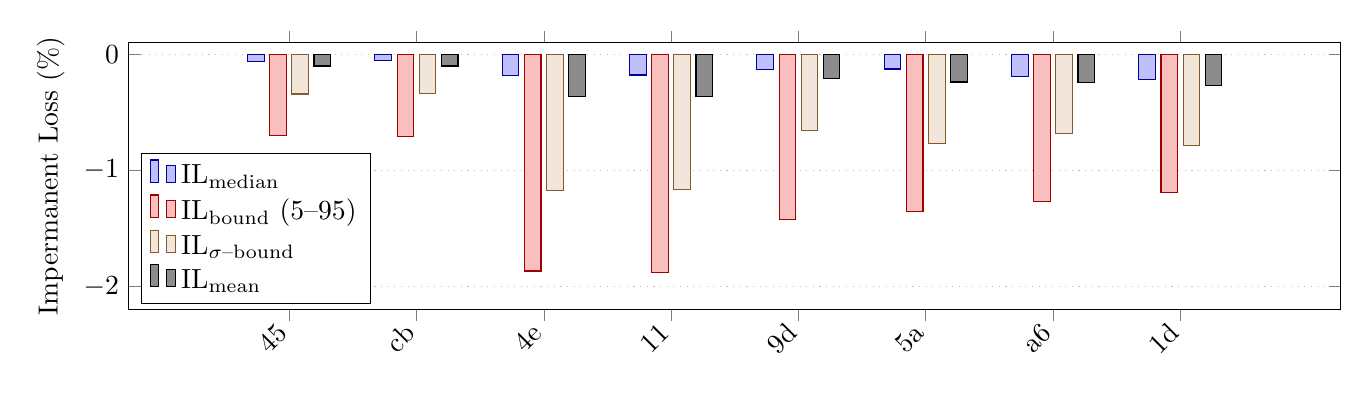
\begin{tikzpicture}
\begin{axis}[
    width=1.4\textwidth,
    height=0.41\textwidth,
    ybar,
    bar width=6pt,
    enlarge x limits=0.18,
    ymin=-2.2, ymax=0.1,
    ymajorgrids=true,
    grid style={dotted},
    ylabel={Impermanent Loss (\%)},
    symbolic x coords={45,cb,4e,11,9d,5a,a6,1d},
    xtick=data,
    xticklabel style={rotate=45, anchor=east},
    legend style={
        at={(0.01,0.02)},
        anchor=south west,
        draw=black,
        fill=white,
        %font=\Large,
    },
    legend cell align={left},
]

% IL_median
\addplot[draw=blue!70!black, fill=blue!25, bar shift=-12pt] coordinates { (45,-0.062025) (cb,-0.053979) (4e,-0.184368) (11,-0.179866) (9d,-0.133229) (5a,-0.127624) (a6,-0.191402) (1d,-0.217280) };
\addlegendentry{$\mathrm{IL}_{\text{median}}$}

% IL_bound (5--95)
\addplot[draw=red!70!black, fill=red!25, bar shift=-4pt] coordinates { (45,-0.698558) (cb,-0.708234) (4e,-1.867968) (11,-1.879260) (9d,-1.420822) (5a,-1.353484) (a6,-1.269196) (1d,-1.191524) };
\addlegendentry{$\mathrm{IL}_{\text{bound}}~(5\text{--}95)$}

% IL_sigma-bound
\addplot[draw=brown!70!black, fill=brown!20, bar shift=4pt] coordinates { (45,-0.343281) (cb,-0.342155) (4e,-1.173647) (11,-1.166907) (9d,-0.655256) (5a,-0.770508) (a6,-0.683694) (1d,-0.786992) };
\addlegendentry{$\mathrm{IL}_{\sigma\text{--}\text{bound}}$}

% IL_mean
\addplot[draw=black, fill=black!45, bar shift=12pt] coordinates { (45,-0.102314) (cb,-0.102141) (4e,-0.367057) (11,-0.366243) (9d,-0.207247) (5a,-0.240038) (a6,-0.242804) (1d,-0.272718) };
\addlegendentry{$\mathrm{IL}_{\text{mean}}$}

\end{axis}
\end{tikzpicture}

}
\caption{Cross-pool comparison of four monthly full-range CPMM proxy IL screening metrics.}
\label{fig:monthly_il_summary_metrics}
\end{minipage}

\end{figure*}

We next summarize the monthly full-range proxy IL distribution using the four screening metrics from Section~\ref{sec:metrics}. Fig.~\ref{fig:monthly_il_summary_metrics} reports $\mathrm{IL}_{\text{median}}$, $\mathrm{IL}_{\text{bound}}~(5\text{--}95)$, $\mathrm{IL}_{\sigma\text{-bound}}$, and $\mathrm{IL}_{\text{mean}}$. These statistics provide an ex-ante screening view of pair-level divergence risk under the common full-range benchmark.
First, in this sample, the metrics consistently separated the pools into clear proxy-risk tiers. The WBTC/WETH pools (45 and cb) exhibited the smallest proxy IL losses across all summaries. Their typical monthly proxy IL was close to zero (medians $\approx-0.062\%$ and $\approx-0.054\%$) and their proxy downside exposure was markedly milder than the rest (5--95 bounds around $-0.70\%$). At the opposite end, the WETH/USDT pools (4e and 11) displayed the largest systematic proxy IL, with the most negative means (both $\approx$ $-0.367\%$) and the deepest proxy downside bounds (5--95 bounds near $-1.87\%$ and $\sigma$-bounds around $-1.17\%$). 
The remaining pools formed an intermediate proxy-risk regime, having medians between roughly $-0.13\%$ and $-0.22\%$. Meanwhile, their proxy downside bounds were substantially less severe than the WETH/USDT group (5--95 bounds between $\approx$ $-1.19\%$ and $-1.42\%$). This indicated meaningfully smaller proxy tail exposure despite non-negligible typical proxy IL.

The second trend was that the four screening metrics emphasized different aspects of proxy IL risk. 
As a result, they could alter the relative ranking within the intermediate tier. 
For example, 1d had the most negative median among the intermediate pools ($\approx-0.217\%$), indicating weaker median-month proxy performance. 
However, its downside bound was the shallowest in that tier (5--95 bound $\approx-1.19\%$), implying comparatively stronger proxy tail protection. 
Conversely, 9d had a less negative median ($\approx-0.133\%$) but a deeper 5--95 bound ($\approx-1.42\%$), reflecting more severe adverse-month proxy exposure. 
Similarly, a6 and 5a had comparable means ($\approx-0.243\%$ and $-0.240\%$) but differed in proxy tail behavior (5--95 bounds $\approx-1.27\%$ versus $\approx-1.35\%$). 
This illustrated that pools could share similar average proxy IL while differing in the severity of rare dislocations.


\begin{figure}[t]
\centering
\resizebox{0.4\textwidth}{!}{%
        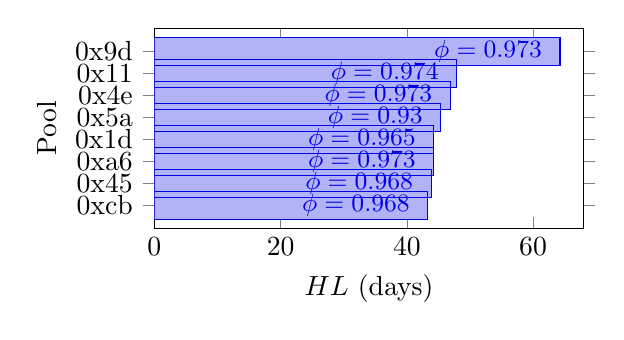
\begin{tikzpicture}
  \begin{axis}[
    xbar,
    width=0.58\textwidth,
    height=0.34\textwidth,
    xlabel={$HL$ (days)},
    ylabel={Pool},
    % order bars by HalfLife (largest at top), matching the new results:
    symbolic y coords={0x9d,0x11,0x4e,0x5a,0x1d,0xa6,0x45,0xcb},
    ytick=data,
    y dir=reverse,
    xmin=0,
    xmax=68,
    bar width=10pt,
    enlarge y limits=0.15,
    point meta=explicit,
    nodes near coords={$\phi=\pgfmathprintnumber[fixed,precision=3]{\pgfplotspointmeta}$},
    nodes near coords style={
        anchor=east,
        xshift=-3pt,
        font=\small
    },
  ]

    % (half-life, pool-id) [mean phi]
    \addplot coordinates {
      (64.26,0x9d) [0.973] % 9d  WBTC/USDT
      (47.89,0x11) [0.974] % 11  WETH/USDT 0.05%
      (46.88,0x4e) [0.973] % 4e  WETH/USDT 0.30%
      (45.39,0x5a) [0.930] % 5a  AAVE/WETH 0.30%
      (44.28,0x1d) [0.965] % 1d  UNI/WETH 0.30%
      (44.28,0xa6) [0.973] % a6  LINK/WETH 0.30%
      (43.84,0x45) [0.968] % 45  WBTC/WETH 0.05%
      (43.33,0xcb) [0.968] % cb  WBTC/WETH 0.30%
    };

  \end{axis}
\end{tikzpicture}

    }
\caption{Mean estimated half-life of log-price-ratio shocks over rolling 180-day windows, together with the corresponding mean AR(1) coefficient $\phi$.}
\label{fig:half_life_180d_mean_phi_inside}
\end{figure}

Fig.~\ref{fig:half_life_180d_mean_phi_inside} presents the mean 180-day rolling $HL$ and AR(1) coefficient $\phi$, computed from overlapping 180-day windows. 
For each pool, we construct an adjusted price series $P_{\text{adj},t}$ (inverted when its mean is below unity) and fit an AR(1) model to the log prices, $Z_t=\ln P_{\text{adj},t}$. 
The window-specific coefficients $\phi_t$ are converted to half-lives via $\mathrm{HL}_t=-\ln 2 / \ln \phi_t$.
Prior to estimating persistence, we perform an Augmented Dickey--Fuller (ADF) test as a basic stationarity diagnostic for the log price-ratio series. 
The resulting half-lives provide reduced-form summaries of relative-price persistence, not structural estimates of AMM dynamics.
The figure shows that price deviations in these markets were persistent, but persistence differed materially across pools. 
The mean $HL$ ranged from $43.33$ to $64.26$ days, while the mean AR(1) coefficients spanned approximately $0.930$ to $0.974$, implying that price-ratio shocks typically decayed over several weeks to roughly two months. 
Because the mapping from $\phi$ to $HL$ is highly nonlinear as $\phi\to 1$, small differences in persistence could translate into meaningful differences in expected shock duration.
This effect was evident in the top-ranked pool 9d (WBTC/USDT), which attained the longest mean $HL$ ($64.26$ days) despite having $\phi\approx0.973$, similar to pools 4e and 11. 
This suggests that near-unit-root episodes in some windows disproportionately increased average $HL$, even when mean $\phi$ values were similar.

Additionally, analyzing the results by pool type revealed a revised cross-sectional pattern.
The WBTC/USDT pool 9d was the most persistent market by a wide margin. 
This implies that deviations between BTC and the dollar-pegged asset could remain sticky for extended periods, potentially sustaining proxy IL exposure over longer horizons.
In contrast, the two WBTC/WETH pools (45, cb) sat at the bottom of the ranking (mean $HL\approx 43$--$44$ days), consistent with faster relative adjustment between two major crypto-assets. 
The WETH/USDT pools (11, 4e) formed an intermediate cluster around $\approx 47$ days, indicating persistence that was substantial but below the BTC--stablecoin case. 
Beyond the stablecoin-based pools, the protocol-token pairs occupied a broader middle band.
Pool 5a (AAVE/WETH) exhibited the lowest mean $\phi$ ($\approx0.930$) yet still had $HL\approx45$ days. 
Pools 1d (UNI/WETH) and a6 (LINK/WETH) were close in $HL$ (both $\approx44.28$ days) despite differing mean $\phi$ values. 
This underscored that average $HL$ could be shaped by the distribution of window-level persistence, not the mean coefficient alone.
Overall, none of the pools exhibited rapid mean reversion. Instead, pair-level shocks tended to decay gradually over the medium term, implying that divergence episodes can remain relevant over realistic LP holding horizons.


\subsection{Recursive Calibration of Proxy IL Metrics}
\label{subsec:backtesting_il}

The IL analysis above provides an \emph{ex post} summary of historical risk under the full-range proxy benchmark. 
To test whether the historical proxy summaries remain informative for subsequent months under the same full-range benchmark, we run a recursive calibration exercise.
For each pool and month $t$ (starting at $t=13$), we estimated the four presented metrics: $\mathrm{IL}_{\text{bound}}$, $\mathrm{IL}_{\sigma\text{-bound}}$, $\mathrm{IL}_{\text{median}}$, and $\mathrm{IL}_{\text{mean}}$. We use an expanding window that included only data prior to month $t$. 
This produced an \emph{ex ante} historical-risk estimate, denoted $\mathrm{IL}^{(t)}_{\text{estimate}}$, which we compare with the realized proxy IL in month $t$, denoted $\mathrm{IL}^{(t)}_{\text{real}}$.
We then computed the exceedance rate $\hat{\alpha}$, the fraction of out-of-sample months where realized proxy IL was worse (more negative) than the historical-risk estimate:
\(
\hat{\alpha}
= \frac{1}{T_{\text{oos}}}\sum_{t=1}^{T_{\text{oos}}}
\mathbf{1}\!\left\{\mathrm{IL}^{(t)}_{\text{real}} < \mathrm{IL}^{(t)}_{\text{estimate}}\right\},
\)
where $T_{\text{oos}}$ is the number of out-of-sample months. 
For a stable distribution, the nonparametric 10\% lower-tail bound should have an exceedance rate near $0.10$. The normal-reference $\sigma$-bound has a one-sided benchmark of approximately $0.16$ under the normal approximation for $\ln R^{(h)}$. The median has a natural exceedance benchmark of $0.50$. The mean does not define a quantile target for a skewed IL distribution, so its exceedance rate is reported descriptively rather than treated as a formal calibration target.

Fig.~\ref{fig:backtest_scores_heatmap} visualized these exceedance rates after converting them into normalized calibration scores to facilitate cross-metric comparison. 
For each metric, we mapped $\hat{\alpha}$ to a unit-scale score in $[0,1]$ based on its deviation from the target exceedance level $\alpha^\star$. 
Under this normalization, a score of $1$ indicated perfect calibration, and lower scores indicated larger deviations from the target.
For the mean metric, the score is included only as a descriptive comparison using $0.50$ as a symmetry benchmark, not as a formal calibration target.
The results show distinct heterogeneity in performance across pools. 
For some pools (e.g., 9d), the 10\% bound ($\mathrm{IL}_{\text{bound}}$) was well-calibrated, yielding $\hat{\alpha}\approx0.093$, close to the theoretical target of $0.10$. 
Conversely, pools such as 45 and cb exhibited higher exceedance rates ($\hat{\alpha}\approx0.186$), indicating that historical proxy summaries tended to underestimate subsequent full-range downside risk. 
Moreover, for most pools, the median exceedance rate fell below $0.50$ (roughly $0.33$--$0.35$), suggesting conservative historical-risk estimates for typical months but weaker coverage of extreme downside events.
This implies that calibration quality is pool-dependent and that tail-oriented proxy metrics can under-cover future full-range proxy IL in the presence of heavy-tailed divergence shocks.

\begin{figure}[b]
    \centering
\includegraphics[width=0.53\textwidth]{backtesting_analysis.tex}
\caption{Normalized recursive-calibration scores for monthly proxy IL metrics across pools, where higher scores indicate closer agreement with the target coverage rate.}
\label{fig:backtest_scores_heatmap}
\end{figure}

\subsection{Stylized Passive Uniswap v3 Simulation and Proxy Alignment}
\label{subsec:stylized_v3_validation}

Recursive calibration evaluates the historical-risk estimates under the common full-range proxy benchmark, but does not show whether the induced pool rankings remain informative after introducing protocol-specific LP mechanics. We therefore evaluate stylized passive Uniswap v3 positions using fixed price bands, daily path-dependent valuation, and in-range fee accrual. This provides a demanding validation setting because concentrated-liquidity outcomes are range-dependent.

\subsubsection{Stylized passive-v3 simulation by pool and band}

For each pool-month, an LP enters at the start-of-month price with normalized initial capital and holds the position without rebalancing until month-end. We evaluate a full-range benchmark and symmetric $\pm20\%$, $\pm10\%$, and $\pm5\%$ bands, representing broad, moderate, and tight passive concentration rather than optimized strategies.

Position inventory and daily valuation follow Section~\ref{subsec:cl_valuation}. Fees accrue only while the position is in range, are allocated according to its active liquidity relative to pool liquidity, and are not reinvested. Monthly excess return is measured relative to a HODL portfolio initialized with the same token amounts. Gas costs, slippage, and active repositioning are excluded.



\begin{table}[t]
\centering
\scriptsize
\begingroup
\setlength{\tabcolsep}{2.3pt}
\renewcommand{\arraystretch}{0.92}

\begin{tabular}{lrrrr}
\toprule
\multicolumn{5}{c}{\textit{(a) Median excess return (\%)}} \\
\cmidrule(lr){1-5}
Pool & Full range & $\pm20\%$ & $\pm10\%$ & $\pm5\%$ \\
\midrule
4e & 2.80 & 0.56 & -1.39 & -3.78 \\
11 & 3.28 & 1.61 & -0.71 & -2.95 \\
9d & 2.24 & 0.92 & -0.07 & -2.80 \\
45 & 1.65 & 0.88 &  0.50 & -0.98 \\
cb & 1.06 & 0.52 & -0.01 & -1.31 \\
5a & 3.24 & 1.54 & -0.12 & -2.51 \\
a6 & 3.77 & 1.12 & -0.28 & -3.34 \\
1d & 1.95 & 0.07 & -2.46 & -4.18 \\
\bottomrule
\end{tabular}

\vspace{3pt}

\begin{tabular}{lcccc}
\toprule
\multicolumn{5}{c}{\textit{(b) Downside and in-range activity}} \\
\cmidrule(lr){1-5}
Pool &
\shortstack{Full range\\$P_{10}$} &
\shortstack{$\pm20\%$\\$P_{10}/A$} &
\shortstack{$\pm10\%$\\$P_{10}/A$} &
\shortstack{$\pm5\%$\\$P_{10}/A$} \\
\midrule
4e & 0.69 & -11.26/81.70 & -14.16/60.54 & -15.61/40.79 \\
11 & 1.23 & -10.41/81.81 & -13.48/60.59 & -15.77/41.02 \\
9d & 0.82 &  -6.60/89.87 &  -9.21/71.43 & -10.63/48.02 \\
45 & 0.59 &  -1.58/95.76 &  -5.11/80.33 &  -6.44/58.02 \\
cb & 0.14 &  -2.66/95.84 &  -5.44/80.94 &  -6.69/58.65 \\
5a & 1.01 &  -5.68/90.61 &  -9.06/67.47 & -10.74/43.24 \\
a6 & 1.36 &  -5.61/86.84 &  -8.90/64.83 & -11.23/42.67 \\
1d & 0.45 &  -6.55/87.52 &  -9.66/64.37 & -11.59/43.43 \\
\bottomrule
\end{tabular}

\endgroup
\caption{Monthly passive-v3 outcomes. (a) Median
excess return. (b) The 10th-percentile outcome
($P_{10}$) and active share ($A$), respectively. All values are
percentages. Full-range activity equals 100\% for every pool.}
\label{tab:stylized_v3_results}
\end{table}

Table~\ref{tab:stylized_v3_results} reveals a consistent passive-concentration tradeoff: Narrower bands reduce median excess returns, worsen downside outcomes, and lower active share. Greater capital efficiency applies only while the position remains in range. Without repositioning, range exits reduce fee accrual and create one-sided inventory exposure.
The effect is milder for the correlated WBTC/WETH pools 45 and cb, which
are the most resilient under the $\pm5\%$ policy, than for the stable--volatile and protocol-token pools. Thus, tighter passive ranges do not mechanically improve realized LP performance.


\subsubsection{Same-Sample Proxy Alignment under Passive Range Concentration}
\label{subsubsec:proxy_vs_realized}

We next compare the pool ranking implied by the proxy layer with the realized ordering produced by the stylized passive Uniswap v3 simulation. Net90 is the tail-adjusted screening score defined in Section~\ref{sec:metrics}. It combines fee yield with a 10th-percentile proxy IL downside term. Here, Net90 is computed over the same pool-month sample used in the v3 simulations. This comparison is therefore a same-sample alignment diagnostic rather than a predictive backtest. It assesses whether the proxy metric captures the cross-sectional pool attractiveness observed under the realized passive-v3 strategies.

Table~\ref{tab:proxy_vs_realized_ranks} presents the same-sample Net90 rank together with the realized ranks under full-range, $\pm20\%$, $\pm10\%$, and $\pm5\%$ bands. The realized ranks are based on median monthly excess return relative to HODL. For both orderings, rank~1 denotes the most attractive pool. It corresponds to the highest Net90 score in the proxy ranking and the highest median monthly excess return in each realized ranking. Fig.~\ref{fig:concentration_breakdown} summarizes the alignment using Spearman rank correlation, which measures whether two orderings rank the pools similarly. Values near $1$ indicate strong agreement, values near $-1$ indicate reversed orderings, and values near zero indicate little monotonic association.

The results show strong agreement under broad passive exposure. The correlation is $0.952$ under full-range exposure and remains high at $0.786$ under the $\pm20\%$ band. These results suggest that the proxy layer captures pool-level fee and inventory-risk tradeoffs that remain relevant when range constraints are weak.

The ranking relationship changes under tighter passive ranges. The Spearman correlation falls to $-0.310$ under both the $\pm10\%$ and $\pm5\%$ bands. This negative association is driven mainly by the WBTC/WETH pools. Pool 45 has Net90 rank~7 but becomes the top-ranked pool under both tighter bands. Pool cb has Net90 rank~8 but rises to realized rank~2. In contrast, pools that rank highly under Net90, such as a6, 5a, and 11, move to lower realized positions once the range becomes tight.

This deterioration is consistent with the active-share patterns reported in Table~\ref{tab:stylized_v3_results}. As ranges narrow, positions spend less time in range. Realized outcomes therefore become more dependent on the price path, the timing of range exits, and the inventory accumulated while the position is inactive. The pool-level fee does not capture these range-specific effects and divergence-risk tradeoff summarized by Net90.

These results delineate the scope of the proxy layer. Net90 remains informative as a first-stage pool-screening metric for full-range and wide passive strategies. Under tight concentration, position activity and path-dependent inventory exposure become increasingly important, making a pool-level divergence-and-fee proxy insufficient on its own. Net90 should therefore be followed by a range-specific evaluation when narrow concentrated-liquidity positions are considered.


\begin{figure*}[t]
\centering
\footnotesize

\begin{minipage}[t]{0.60\textwidth}
\vspace{0pt}
\centering
\begin{tabular}{lccccc}
\toprule
Pool & Net90 rank & Full-range & $\pm20\%$ & $\pm10\%$ & $\pm5\%$ \\
\midrule
a6 & 1 & 1 & 3 & 5 & 6 \\
5a & 2 & 3 & 2 & 4 & 3 \\
11 & 3 & 2 & 1 & 6 & 5 \\
9d & 4 & 5 & 4 & 3 & 4 \\
4e & 5 & 4 & 6 & 7 & 7 \\
1d & 6 & 6 & 8 & 8 & 8 \\
45 & 7 & 7 & 5 & 1 & 1 \\
cb & 8 & 8 & 7 & 2 & 2 \\
\bottomrule
\end{tabular}
\captionof{table}{Same-sample Net90 ranks versus realized passive-v3 ranks. Rank~1 denotes the most favorable outcome.}
\label{tab:proxy_vs_realized_ranks}
\end{minipage}
\hfill
\begin{minipage}[t]{0.36\textwidth}
\vspace{0pt}
\centering
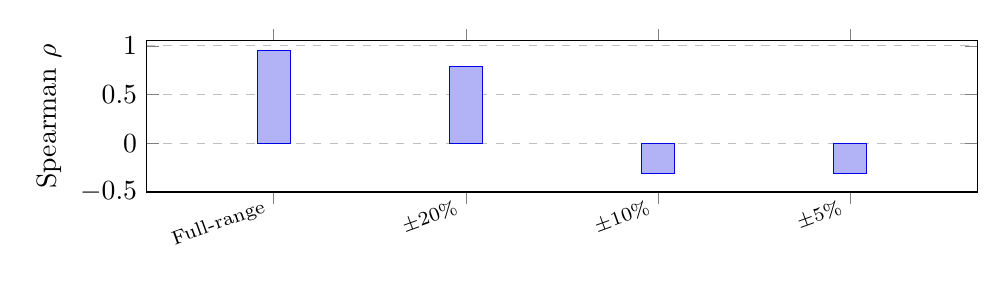
\begin{tikzpicture}
\begin{axis}[
    ybar,
    bar width=12pt,
    width=\textwidth,
    height=3.5cm,
    ymin=-0.50,
    ymax=1.05,
    ylabel={Spearman $\rho$},
    symbolic x coords={Full-range,$\pm20\%$,$\pm10\%$,$\pm5\%$},
    xtick=data,
    xticklabel style={font=\scriptsize, rotate=20, anchor=east},
    ymajorgrids=true,
    grid style=dashed,
    enlarge x limits=0.22,
]
\addplot coordinates {
    (Full-range,0.952)
    ($\pm20\%$,0.786)
    ($\pm10\%$,-0.310)
    ($\pm5\%$,-0.310)
};
\end{axis}
\end{tikzpicture}
\caption{Spearman rank correlation between same-sample Net90 ranks and
realized passive-v3 ranks across range widths.}
\label{fig:concentration_breakdown}
\end{minipage}

\end{figure*}


\section{Discussion: Scope and Implications of Proxy-Based LP Screening}
\label{sec:discussion}

The empirical analysis positions the proposed metrics as a general LP screening layer rather than a Uniswap-v3-specific strategy model. The following subsections outline three key implications of this approach.

\subsection{From Proxy Metrics to Pool Screening}

The proxy metrics capture complementary dimensions of LP risk: Price-ratio divergence, fee compensation, and shock persistence. A key empirical finding is that divergence risk stems from relative-price dynamics rather than isolated token volatility. In our sample, the correlated WBTC/WETH pairs therefore exhibit lower proxy IL than the stable--volatile pools, making pair-level co-movement an important screening variable. This does not imply that correlated pools are inherently superior, because profitability also depends on fee generation, liquidity depth, and tail events.

Furthermore, because average outcomes can mask severe tail dislocations, downside-aware metrics---such as the 10th-percentile proxy IL term in Net90---are important. Shock persistence, measured through AR(1) half-lives, also indicates that relative-price deviations can decay over several weeks, highlighting the importance of matching LP holding horizons to the estimated persistence of divergence risk.

\subsection{Fee Velocity Rather Than Fee Tier}

Fee tier alone is insufficient for assessing LP compensation. A 0.05\% pool requires six times the turnover of a 0.30\% pool to match its fee yield, and more than six times to exceed it. This makes \emph{fee velocity} the relevant screening quantity:
\[
y^{\mathrm{fee}}_t
\approx
\mathrm{FeeTier}
\cdot
\frac{\mathrm{Volume}_t}{\mathrm{TVL}_t}.
\]
This expression separates unit fee margin from capital turnover. High raw volume does not ensure high turnover when TVL is also large, while a high-fee pool can underperform when deep liquidity dilutes its fee yield. Net90 incorporates the resulting fee yield alongside downside proxy IL, thereby evaluating tail-adjusted compensation rather than either component in isolation.

\subsection{Implications for LP Strategy Design}

The same-sample analysis shows that Net90 rankings align closely with realized excess-return rankings under full-range and wide passive bands. Under these weak range constraints, pool and fee-tier selection remain the primary decisions, making the proxy layer informative.

Under tight passive bands, however, this alignment deteriorates. Narrow ranges increase inactivity, reducing fee accrual and introducing one-sided inventory exposure. These range-specific effects are not captured by full-range proxy IL and can dominate the original pool-level tradeoff.

This suggests a two-stage LP strategy design: (1) Use the proposed metrics to screen pools with attractive fee--divergence profiles,  (2) Evaluate protocol-specific parameters such as range selection, active share, rebalancing, gas costs, slippage, and path-dependent inventory exposure. The framework does not claim that full-range CPMM IL exactly values every concentrated position or that the passive-v3 simulations cover all possible strategies. It provides a general screening layer intended to complement, rather than replace, detailed protocol-specific LP models.

\section{Conclusion}
\label{sec:conclusion}
In this paper, we develop a data-driven pool-screening framework that equips LPs with a practical way to quantify IL risk beyond simple fee-tier heuristics.
Using multi-year pool data, we show that net outcomes are driven by the interaction of fee generation and divergence risk, motivating simple selection rules based on distributional IL summaries, tail bounds, and predictability diagnostics. 
The stylized passive-v3 analysis shows that these proxy metrics remain informative for full-range and wide passive exposure, but become less sufficient under tight concentration, where range inactivity can dominate.
Future work will extend the analysis to a broader pool universe across additional DeFi platforms and develop protocol-specific range-selection and adaptive fee policies that adjust to time-varying IL risk.



\bibliographystyle{IEEEtran}
\bibliography{references}

\end{document}